\documentclass[tikz, border=2pt]{standalone}
\usepackage{amsmath}

\begin{document}
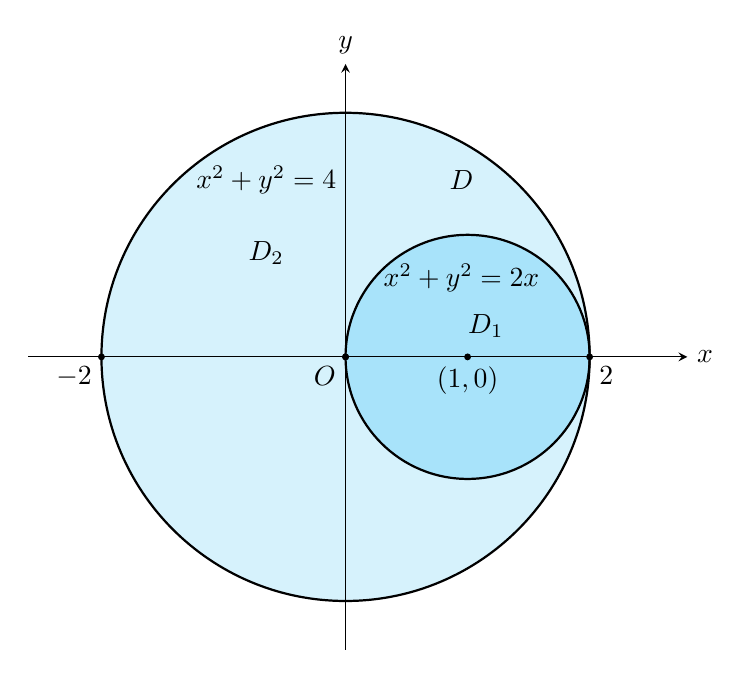
\begin{tikzpicture}[scale=1.55, >=stealth]
    \fill[cyan!16] (0,0) circle (2);
    \fill[cyan!34] (1,0) circle (1);

    \draw[->] (-2.6, 0) -- (2.8, 0) node[right] {$x$};
    \draw[->] (0, -2.4) -- (0, 2.4) node[above] {$y$};

    \draw[thick] (0,0) circle (2);
    \draw[thick] (1,0) circle (1);

    \fill (0,0) circle (0.8pt) node[below left] {$O$};
    \fill (2,0) circle (0.8pt) node[below right] {$2$};
    \fill (-2,0) circle (0.8pt) node[below left] {$-2$};
    \fill (1,0) circle (0.8pt) node[below] {$(1,0)$};
    \fill (0,0) circle (0.8pt);

    \node at (0.95, 1.45) {$D$};
    \node at (1.15, 0.25) {$D_1$};
    \node at (-0.65, 0.85) {$D_2$};

    \node at (-0.65, 1.45) {$x^2+y^2=4$};
    \node at (0.95, 0.65) {$x^2+y^2=2x$};
\end{tikzpicture}
\end{document}
